\chapter{Search Scaling for Web-Scale Recommendations}
\label{ch:scale-efficient-retrieval}

\section{Introduction}

Chapters~\ref{ch:universal-video-retrieval} and~\ref{ch:spatiotemporal-scaling} address what a video embedding should represent and how visual evidence should be supplied to it. Accurate embedding generation is still insufficient when the learned relevance signal must be evaluated over billions of candidates under strict latency and throughput constraints~\cite{zhu2018learning,liu2021jizhi}. This chapter addresses this final bottleneck, search scaling, through the joint design of the learned metric, graph traversal, and GPU execution. The relevant background is reviewed centrally in \S\ref{sec:bc-search} and \S\ref{sec:lr-search}.

Retrieval-and-ranking frameworks~\cite{cheng2016wide,ma2020off} reduce a massive item catalog to a compact candidate set before ranking and are widely used in industrial systems~\cite{covington2016deep,borisyuk2016casmos,eksombatchai2018pixie}. The retrieval stage must preserve relevance while avoiding exhaustive scoring, making the interaction between metric quality and search efficiency central to deployment-scale retrieval.

This chapter focuses on the retrieval stage in Baidu's web-scale recommendation scenarios, e.g., news feed, Tieba, and video clips. Recent works~\cite{tan2020fast,chen2022approximate} establish the retrieval framework in a training-and-search manner.
Based on the complex relational dependencies modeling ability of Deep Neural Network~(DNN)~\cite{zhang2019deep}, they attempt to train a DNN-based metric for more accurate user-item relevance estimation compared with simple functions~\cite{dehghani2017neural,tay2018latent}.
Nevertheless, real-time retrieval is difficult due to complicated neural computations on massive candidates.
To solve the problem, researchers have been exploring the potential of Approximate Nearest Neighbor Search~(ANNS) algorithms to mitigate extensive computations, which search for relatively relevant items for each query user by selectively visiting instead of the entire item base.
Early works propose tree-based ANNS to organize data points in a tree-like structure by recursively splitting the dimensional space~\cite{friedman1977algorithm}.
However, they underperform in web-scale recommendations that aim to retrieve divergent and high-dimensional information because they are sensitive to complex feature spaces and item relationships~\cite{wang2021comprehensive}.
To improve retrieval effectiveness, the latest frameworks leverage graph-based ANNS algorithms that build similarity-based candidate graphs to efficiently expand the candidate set via graph traversal.
For example, HNSW~\cite{malkov2018efficient} hierarchically establishes a multi-layer indexing graph, grounding coarse-to-fine navigation towards the most satisfactory candidates.


However, we confront three challenges in developing an accurate and efficient retrieval framework for web-scale recommendations.
\textit{(1)~Unified modeling of multi-relational user-item relevance.} Baidu recommendation applications consist of dozens of distinct and related behaviors~(e.g., click, browse) that are typically modeled by a tailored metric for estimating relevance between users and items. However, the independent modeling of these user-item interactions fails to capture the semantic relations of diverse user behaviors, which are mutually beneficial between them~\cite{tan2020fast}. Besides, training multiple behavior-specific metrics incurs exponential efforts in system updates. Thus, the first challenge lies in cost-effective multi-relational metric joint training for more accurate relevance estimation.
\textit{(2)~Efficient search on large-scale graph item base.} Baidu devises Graph-based ANNS to traverse relevant candidate items from a graph item base. Practically, a trade-off problem arises that increasing the online retrieval throughput will restrict the search efforts, \ie, the graph traversal steps. However, existing methods make delivering satisfactory items in limited steps difficult, especially for billion-scale graphs in web-scale recommender systems.
On the one hand, neural relevance metrics often violate the triangle inequality, weakening the geometric consistency that supports efficient proximity-graph navigation~\cite{chen2022approximate}. This mismatch can force the exploration of redundant edges, decreasing the possibility of reaching distant yet relevant candidates.
On the other hand, graph-based ANNS usually search for relevant items greedily, which may be stuck in a narrow space after a short-length traversal among a large-scale graph.
The inability to balance search depth and breadth degrades the quality of real-time recommendations. Addressing this challenge requires developing a search-compatible relevance metric and a deep-and-broad traversal algorithm for efficient graph search.
\textit{(3)~Accelerating irregular neural computation in high concurrency.} At Baidu, users raise hundreds of millions of recommendation requests per second. These request executions are irregular because divergent user profiling drives distinct search paths, where the visited items should be estimated for their relevance by the neural metric. Baidu has developed a GPU-accelerated framework for web-scale recommendations to leverage the computational economy of GPUs~\cite{liu2022lion}. However, their performance degrades under highly concurrent, non-uniform workloads because of frequent kernel launches, a process with fixed latency overhead that dominates runtime when computations are small and irregular~\cite{el2016klap}. Millions of sequential processes of deep relevance computations on a GPU cluster introduce bottlenecks of recommendation throughput. Therefore, the third challenge is redesigning computation scheduling to accelerate large-scale irregular neural computations for higher throughput.

\begin{figure}[t]
    \centering
    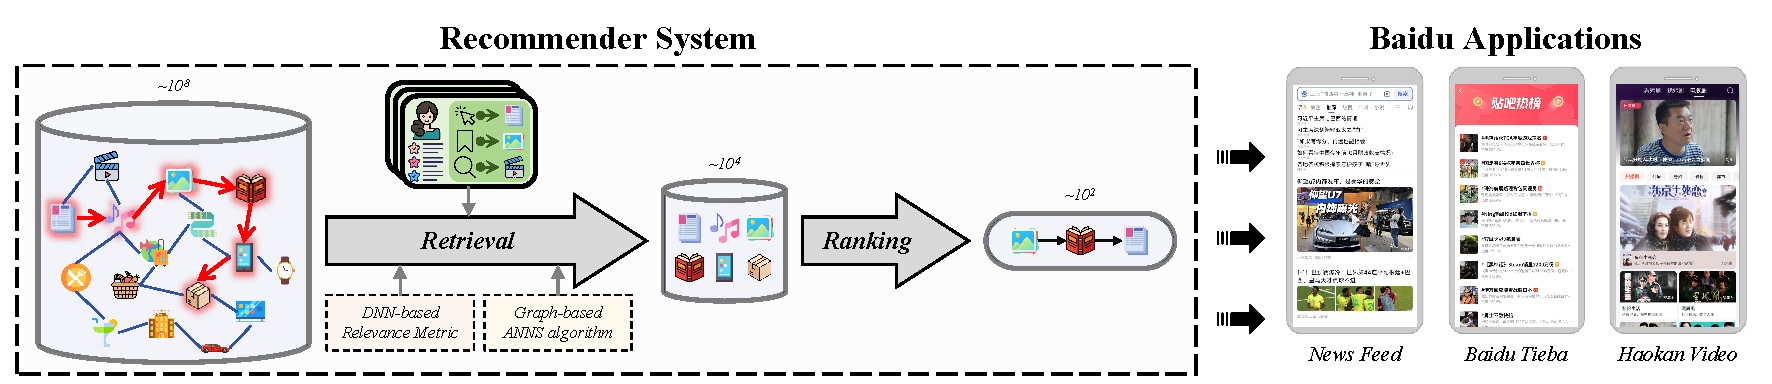
\includegraphics[width=\linewidth]{figures/gmpgr/Application.pdf}
    \caption{Applications of recommender systems at Baidu.}
    \label{gmpgr:fig:application}
\end{figure}

For the application scenarios shown in Figure~\ref{gmpgr:fig:application}, we propose a \textbf{GPU-accelerated Multi-relational Parallel Graph Retrieval~(GMP-GR)} framework for effective and efficient retrieval in web-scale recommendations.
Specifically, we first devise a \textit{Multi-relational User-Item Relevance Metric Learning~(MUIRML)} to generate a practical DNN-based metric via multi-objective optimization.
The metric extracts multi-relational knowledge in inter-dependent user behaviors to capture nuanced user preferences for accurate relevance measurement.
We also use a self-covariant loss to align the ranking regularity of our metric with Euclidean distance, encouraging shorter navigation paths on large graphs.
Second, we design a \textit{Hierarchically Parallel Approximate Nearest Neighbor Search~(HiPANNS)} algorithm to achieve timely and accurate retrieval for highly concurrent queries.
HiPANNS broadens the search space of the large graph item base by divergent parallel and co-optimized search processes, which can efficiently generate more relevant candidates in real-time retrieval.
Based on it, HiPANNS accelerates irregular neural computations from asynchronous requests by adaptive aggregation in a GPU-based cluster for higher retrieval throughput.
In Baidu recommendation applications, we further apply several system optimization strategies, including traffic dispersal, compilation optimization, model quantization, and timely stream update.
Extensive experiments demonstrate the superior retrieval effectiveness and efficiency of GMP-GR in offline retrieving evaluations and online recommendation services.
Our framework has been deployed in more than twenty web-scale recommender systems at Baidu, where it efficiently handles hundreds of millions of requests per second, improving user time-on-page by more than $3\%$ for hundreds of millions of users.

The contributions of this chapter are summarized as follows:
(1)~We propose a GPU-accelerated Multi-relational Parallel Graph Retrieval framework to achieve accurate and efficient retrieval for web-scale recommendations.
(2)~We devise a DNN-based metric to estimate user-item relevance via capturing inter-dependency among complex user-item relations, which can also improve the search efficiency on a large-scale graph for shorter navigation.
(3)~We design a GPU-accelerated parallel graph-based ANNS algorithm for highly concurrent retrieval by billion-scale breadth-depth balanced graph search and parallel irregular computations with adaptive aggregation.
(4)~We conduct extensive experiments to demonstrate retrieval effectiveness and efficiency improvements in offline and online recommendations at Baidu.


\section{Preliminaries}

Baidu has developed a recommendation framework as a comprehensive funnel mechanism to efficiently retrieve and rank items for users from a web-scale database for over twenty internet products~(e.g., news feed, short video clips, search engine, and online advertising)~\cite{liu2021jizhi}.
The recommendation framework has served hundreds of millions of online recommendation requests per second for hundreds of millions of users.
Next, we detail the retrieval framework for Baidu recommendations, including the retrieval problem and the retrieval pipeline.

\subsection{Online Retrieval at Baidu}
This setting instantiates the unified ranking problem in \S\ref{sec:bc-vr} at deployment scale. A user request serves as the query, the item base serves as the candidate corpus, and the learned relevance value determines the top-$K$ ordering. The notation below is specific to the industrial recommendation setting.

Given a user set $\mathcal{U}=\{u_1,u_2,\cdots,u_{N_u}\}$ and an item set $\mathcal{V}=\{v_1,v_2,\cdots,v_{N_v}\}$, consider a query from a user $u$ with raw feature $x_{u}$. The objective of the retrieval stage is to recommend the top-$K$ items that are most relevant to $u$ in order.
Specifically, we define the retrieval problem as a function $\mathcal{F}(\cdot;\cdot)$ that generates a set $V_{u}$ based on the user features. $V_u$ contains the $K$ most similar items $V_{u} = \{v_{u,1},v_{u,2},\cdots,v_{u,K}\}$ as
\begin{equation}
    V_{u} = \mathcal{F}(x_{u};\{v_1,v_2,\cdots,v_{N_v}\}).
\end{equation}

\subsection{Retrieval Pipeline at Baidu}

Baidu has constructed a graph retrieval framework in their recommendation system, including two stages: offline training and online search~\cite{tan2020fast,chen2022approximate}.

\subsubsection{Step 1. Offline Training}
The first stage aims to learn user and item embeddings associated with a relevance metric for estimating the relevance between users and items.
Embeddings and the metric are learnable modules stored by the system, which are immutable in the search stage.
We can also periodically re-train the modules once the properties change significantly.
Overall, the pipeline of the training step is presented below.

\textit{(1)~Users and item feature construction.}
We first prepare the raw features of the users and items that are denoted as $\{x_{u_1},x_{u_2},\cdots,x_{N_u}\}$ and $\{x_{v_1},x_{v_2},\cdots,x_{N_v}\}$, where $N_u$ and $N_v$ are the numbers of users and items, respectively. Meanwhile, the interaction records of users $u$ and items $v$ are denoted as $\{D^z_{u,v}\}$. For an interaction type $z$, $D^z_{u_i,v_j}$ is the interactive value between a user $u_i$ and an item $v_j$, which reflects how close they are in terms of the interaction $z$.

\textit{(2)~User and item embedding projection.}
Then, we pre-define a user and an item projector, $\mathcal{H}_u(\cdot)$ and $\mathcal{H}_v(\cdot)$, to transform raw features into learnable embeddings as user and item representations, which are defined as $h_{u_i} = \mathcal{H}_u(x_{u_i})$ and $h_{v_j} = \mathcal{H}_v(x_{v_j})$.

\textit{(3)~User-item relevance metric definition.}
After that, we devise a DNN-based learnable metric~\cite{dehghani2017neural,tay2018latent} to estimate the relevance between a user and an item by a high-dimensional calculation of their embeddings.
Hence, we aim to obtain a metric $\Delta(\cdot,\cdot)$ to quantify the relevance value given a user embedding and an item embedding as
\begin{equation*}
\delta_{u,v} = \Delta(h_u,h_v).
\end{equation*}

\textit{(4)~Optimization of embeddings and the metric.}
Next, we optimize the user embeddings, item embeddings, and the relevance metric based on the user features, item features, and user-item interactions. We describe the optimization as a function $\mathcal{F}_t(\cdot,\cdot,\cdot)$ that
\begin{equation}
    \{h_u\}, \{h_v\}, \Delta(\cdot,\cdot) = \mathcal{F}_t(\{x_u\}, \{x_v\}, \{D^z_{u,v}\}).
\end{equation}
The learned embeddings and the relevance metric are used in the online search stage to measure user-item relevance. 

\begin{figure}[t]
    \centering
    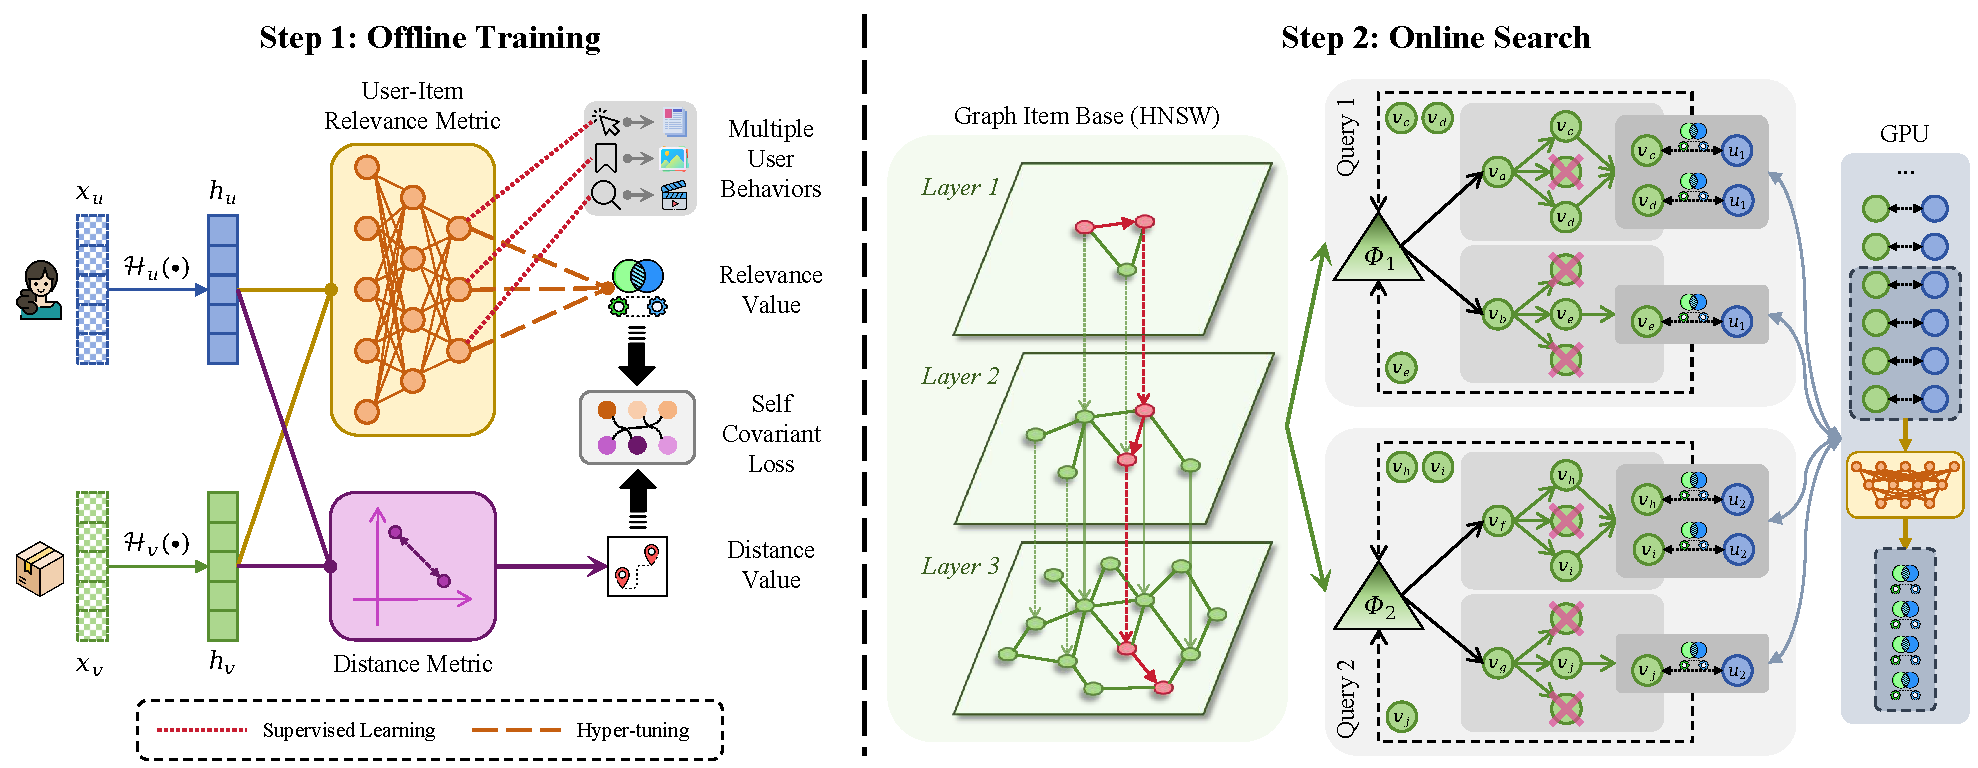
\includegraphics[width=\linewidth]{figures/gmpgr/GMP-GR.pdf}
    \caption{An overview of the GPU-accelerated Multi-relational Parallel Graph Retrieval framework.}
    \label{gmpgr:fig:gmp-gr}
\end{figure}


\subsubsection{Step 2. Online Search}
In the second stage, we construct a graph-based item database that supports an efficient search for the target items.
Traditional tree-based ANNS fails to handle web-scale data with high dimensions and uneven distributions, and requires extensive tree construction costs.
Instead, we follow graph-based ANNS to construct a graph item base that can efficiently navigate possibly relevant items and retrieve satisfactory items for given users based on graph search.
Specifically, we adopt HNSW~\cite{malkov2018efficient} as the graph structure.
HNSW utilizes a multi-layered graph structure, denoted as a $L$-layer graph $G$, where each upper layer contains fewer nodes to facilitate efficient search paths. Based on its hierarchy, we can effectively narrow the search space for nearest neighbors in the base layer, initiating the search process from the upper layers.

In the online search, we infer $K$ relevant items with a querying user as follows. We perform the search iteratively across each layer of the HNSW structure, with the selected items from one layer serving as seed nodes for traversal in the subsequent layer. For each layer, we first access the corresponding user embedding. Second, we generate seed nodes, from which we start to traverse the graph. Third, we expand the candidate node set by visiting neighbors of existing nodes and continuously update the most similar ones for the queried user. The $K$ most similar items are ultimately extracted from the final layer.
The overall search process for the relevant item set $\hat{V}_u$ for user $u$ can be defined as
\begin{equation}
    \hat{V}_u = \mathop{\arg\max}\limits_{\substack{V_u \subseteq \mathcal{V} \\ |V_u|=K}} \sum\limits_{v \in V_u} \delta_{u,v}.
\end{equation}


\section{GPU-accelerated Multi-relational Parallel Graph Retrieval Framework}

This section introduces the GPU-accelerated Multi-relational Parallel Graph Retrieval~(GMP-GR) framework deployed at Baidu for web-scale recommendation.
As shown in Figure~\ref{gmpgr:fig:gmp-gr}, GMP-GR equips two main modules to achieve effective and efficient performance.
In the training step, multi-relational user-item relevance metric learning generates a DNN-based metric that captures inter-dependent relationships between users and items while encouraging Euclidean ranking regularity for path-efficient graph search.
In the search step, a hierarchically parallel graph-based ANNS algorithm effectively delivers reliable search candidates in high concurrency, which explores a breadth-depth balanced search space and synchronizes large-scale irregular neural computations on GPUs.


\subsection{Multi-relational User-item Relevance Metric Learning}\label{gmpgr:sec:metric}

The training step aims to optimize the user and item embeddings with the DNN-based metric to model the relevance between users and items.
However, existing DNN-based metrics may model nuanced user preferences incompletely because they incorporate only part of the multi-dimensional behaviors on items, or may lack the geometric regularity that supports efficient graph-based ANNS navigation.
Therefore, we propose a \textit{Multi-relational User-Item Relevance Metric Learning~(MUIRML)} algorithm to train a relevance metric that not only ensures elaborate multi-relational modeling, but also enhances navigating efficiency in the search step, ultimately improving the retrieval effectiveness.

\textit{(1)~DNN-based Relevance computation.}
We first utilize a Multi-Layer Perceptron~(MLP) to model multiple interactive behaviors.
Initially, the input consists of the user embedding $h_u$, the item embedding $h_v$, and the serendipity vector $\tilde{h} \sim \mathcal{N}(0,1)$ for diverse exploration as
\begin{equation}
    h_{u,v}^{(0)} = \operatorname{concat}(h_u+\tilde{h},h_v),
\end{equation}
the MLP inputs $h_{u,v}^{(0)}$ and aims to output the interaction vector $Z_{u,v}$ that stacks multiple interactions $z_{u,v}$ between user $u$ and item $v$.
The overall operation can be defined as
\begin{equation}
    \hat{Z}_{u,v} = \operatorname{MLP}(h_{u,v}^{(0)}),
\end{equation}
where $\hat{Z}_{u,v}$ is the predicted interaction vector.
Specifically, we define the computation of the $m$-th layer MLP as
\begin{equation}
    h_{u,v}^{(m)} = \mathbf{W}^{(m)} \cdot h_{u,v}^{(m-1)}+b^{(m)},
\end{equation}
where $h_{u,v}^{(m)}$ is the $m$-th layer joint representation of user $u$ and item $v$, and $\mathbf{W}^{(m)}$ and $b^{(m)}$ are the $m$-th layer learnable parameters.

Then, we leverage an attention mechanism to aggregate predicted interaction values for a joint understanding of diverse user behaviors.
Specifically, the attention vector $\mathbf{A}$ is multiplied on $\hat{Z}_{u,v}$ to produce the final user-item relevance value $\delta_{u,v}$ as
\begin{equation*}
\delta_{u,v} = \mathbf{A} \cdot \hat{Z}_{u,v}.
\end{equation*}
where $\mathbf{A}$ is initialized with $\frac{1}{|\mathbf{A}|}$ and can be hyper-tuned to achieve personalized behavior importance for different web recommendation scenarios.


\textit{(2)~Self-supervised loss for short graph navigation.}
Instead of directly forcing the alignment between user-item relevance values computed by the DNN-based metric and Euclidean distance, we encourage the DNN-based metric to follow the ranking regularity of Euclidean distance.
Specifically, we devise a Self Covariant Loss~(SCL) to quantify the gap of the ranking regularity via the divergence of the pairwise values covariance for two metrics.
By minimizing the loss, the order of items ranked according to our metric will be similar to the Euclidean distance, while the relevance values will be maximally retained for accurate estimation by multi-dimensional understanding.
In this way, we can eliminate unnecessary traversal paths and increase the possibility of approaching the optimal candidates.

Specifically, we randomly sample $N_l$ pairs of users and items $\{(u_{i_1},v_{j_1}),\cdots,(u_{i_{N_l}},v_{j_{N_l}})\}$ and compute their DNN-based relevance values $\{\delta_{u,v}\}$ and Euclidean distance $\{\delta^{\prime}_{u,v}\}$, respectively. Then, we calculate the correlation of two groups of values based on their covariance as
\begin{equation}
    \rho_{u,v} = {\frac {\sum \limits _{k=1}^{N_l}(\delta_{u_k,v_k}-{\overline {\delta_{u,v}}})(\delta^{\prime}_{u_k,v_k}-{\overline {\delta^{\prime}_{u,v}}})}{{\operatorname{VAR}(\delta_{u,v})} \cdot {\operatorname{VAR}(\delta^{\prime}_{u,v})}}},
\end{equation}
where $\operatorname{VAR}(x)=\sqrt {\sum_{k=1}^{N_l}(x-{\overline {x}})^{2}}$.


\textit{(3)~Multi-objective optimization for embeddings and the relevance metric.}
Lastly, we design the multi-objective optimization to train the user and item embeddings, as well as the DNN-based relevance metric. The loss is defined as
\begin{equation}
    \mathcal{L} = \sum\limits_{i=1}^{N_u} \sum\limits_{j=1}^{N_v} (\Vert Z_{u_i,v_j} - \hat{Z}_{u_i,v_j} \Vert_2 + \sum\limits_{k=1}^{N_l} \frac{1}{\rho_{u_{i_k},v_{j_k}}+1}),
\end{equation}
which will be optimized by gradient-based algorithms.
In this way, we can simultaneously minimize the prediction error of multi-relational interaction behaviors and maximize the similarity between the ranking regularities of our DNN-based metric and Euclidean distance, which can generate shorter graph-search paths for more efficient retrieval.


\subsection{GPU-accelerated Hierarchically Parallel Approximate Nearest Neighbor Search}\label{gmpgr:sec:search}

In this work, the search step aims to retrieve the most similar items using graph-based ANNS.
Existing graph retrieval frameworks struggle to achieve low-latency retrieval in high-concurrency scenarios for two reasons.
First, their traversal strategies underperform at scale, as they inadequately balance search depth, \ie, refinement of local neighborhoods, and breadth, \ie, coverage of global graph regions, within constrained computational budgets~\cite{ootomo2024cagra}.
Second, the underlying GPU-based infrastructure faces inefficiencies when handling asynchronous retrieval requests, which includes tremendous irregular neural computations according to divergent search routes. The frequent kernel launch of GPU computation from different queries induces significant overhead and contention under extreme concurrency~\cite{pan2023recom}.
These limitations collectively degrade the retrieval throughput for real-time recommendations.
To this end, we propose a \textit{Hierarchically Parallel Approximate Nearest Neighbor Search~(HiPANNS)} algorithm to efficiently answer highly concurrent retrieval queries.
Specifically, HiPANNS consists of two sub-algorithms, \ie, inter-candidate HiPANNS and inter-query HiPANNS.

Inter-candidate HiPANNS~(C-HiPANNS) allows parallel search within the large-scale graph item base to broaden the global search space for more comprehensive retrieval.
For each query $u$, we aim to execute $k$ parallel search processes with different initial seeds $S$.
Each search process traverses the graph item base by visiting the most relevant neighbors.
We jointly maintain candidates by a shared max heap $\Phi_u$ that ranks $k$ current most relevant items among processes.
In this work, we carry out the multi-processing at each layer of the HNSW graph, seeded with top-$k$ candidates ranked by $\Phi_u$ of the last layer.
The parallelized traversal achieves a $k$-fold expansion of the search space, which yields more effective retrieval results.

Inter-query HiPANNS~(Q-HiPANNS) adaptively aggregates irregular neural computations for more efficient GPU-accelerated retrieval against launch bound from extreme concurrency.
We adaptively synchronize the irregular user-item relevance evaluation by a queuing aggregation scheme and parallelize batched neural computation on GPU for acceleration.
First, we initialize a queue $\Psi$ to persistently listen to neural computations. $\Psi$ will record the computations orderly for the following sequential batching, \ie, the element received first will be batched first. Each element in $\Psi$ is produced from C-HiPANNS as a group of $(u,v)$ pairs for measuring neighbor embedding similarity. We dynamically generate batches for parallel computing the GPU cluster $U$.
However, the elements of $\Psi$ vary in amounts due to divergent connections in the graph item base, causing difficulties in aggregating fixed batches that are beneficial to fully utilize the computational ability of GPUs.
To address that, we synthesize batches by adaptively slicing $(u,v)$ groups to fit certain configurations.
Specifically, we set the maximum size of the computing batch as $B_U$. If the size of current batch $B_i$, $N_{B_i}$, is larger than the remaining space $\epsilon$, we split it into two elements, including $B_i^{[1,\epsilon]}=\{(u_{i,1},v_{i,1}),\cdots,(u_{i,\epsilon},v_{i,\epsilon})\}$ and $B_i^{[\epsilon+1,N_{B_i}]}=\{(u_{i,\epsilon+1},v_{i,\epsilon+1}),\cdots,(u_{i,N_{B_i}},v_{i,N_{B_i}})\}$. $B_i^{[1,\epsilon]}$ will be computed in the current executive round of $U$ while $B_i^{[\epsilon+1,N_{B_i}]}$ will be computed in the next.
The output values will be returned as estimations of the relevance between users and items during the processes of C-HiPANNS.

The complete procedures of C-HiPANNS and Q-HiPANNS are summarized in
Algorithms~\ref{gmpgr:alg:c_hipanns} and~\ref{gmpgr:alg:q_hipanns}, respectively.

\begin{algorithm}[t]
    \caption{Inter-candidate HiPANNS.}
    \label{gmpgr:alg:c_hipanns}
    \LinesNumbered
    \KwIn{Query user $u$, HNSW $G$, neighbor hops $T$, heap size $K$, and number of HNSW layers $L$.}
    \KwOut{Top-$K$ retrieved items $V_u$.}
    \Fn{\CHIPANNS{$u$,$G$,$T$,$K$,$L$}}{
        Initialize a $K$-size max heap $\Phi_u$\;
        Initialize $K$ search seeds $S^{(0)}=\{v^{(0)}_{1},v^{(0)}_{2},\cdots,v^{(0)}_{K}\}$ and push them into $\Phi_u$\;
        \For{$l=1,\cdots,L$}{
            Initialize search seeds for the $l$-th layer as $S^{(l)}=\Phi_u$\;
            \ForEach{$v^{(l)}_{i} \in S^{(l)}$ in parallel}{
                \For{$t=1,\cdots,T$ in batch}{
                    Retrieve the $t$-hop neighbor set $\{v^{(l)}_{i,t_j}\}$ of $v^{(l)}_{i}$\;
                    Calculate the relevance $\delta_{u,v^{(l)}_{i,t_j}}$ by \QHIPANNS{$\{(u,v^{(l)}_{i,t_j})\}$}\;
                    Push $v^{(l)}_{i,t_j}$ into $\Phi_u$\;
                }
            }
        }
        \Return{$\Phi_u$}
    }
\end{algorithm}

\begin{algorithm}[t]
    \caption{Inter-query HiPANNS.}
    \label{gmpgr:alg:q_hipanns}
    \LinesNumbered
    \KwIn{GPU cluster $U$ and its batch size $N_U$.}
    \KwOut{Relevance values $\delta_{B_i}$.}
    \Fn{\QHIPANNS{$B_i$}}{
        Initialize an empty $N_U$-size batch $B_U$ and current batch length $N^{\prime}_U=0$\;
        Initialize a queue $\Psi$\;
        Listen to a batch $B_i=\{(u_{i,1},v_{i,1}),\cdots,(u_{i,N_{B_i}},v_{i,N_{B_i}})\}$ in real time and push it into $\Psi$\;
        \ForEach{$B_i \in \Psi$}{
            $\epsilon = N_U - N^{\prime}_U$\;
            \eIf{$N_{B_i} \leq \epsilon$}{
                Concatenate the batch as $B_U = B_U \cup B_i$ and set $N^{\prime}_U = N^{\prime}_U + N_{B_i}$\;
                Calculate $\delta_{B_i}$ on $U$\;
            }{
                Split $B_i$ into $B_i^{[1,\epsilon]}$ and $B_i^{[\epsilon+1,N_{B_i}]}$\;
                Concatenate the batch as $B_U = B_U \cup B_i^{[1,\epsilon]}$\;
                Calculate $\delta_{B_i}$ on $U$\;
                Set $B_U = B_i^{[\epsilon+1,N_{B_i}]}$ and $N^{\prime}_U = N_{B_i} - \epsilon$\;
            }
        }
        Concatenate $\delta_{B_i}$ if $B_i$ is split\;
        \Return{$\delta_{B_i}$}
    }
\end{algorithm}

\section{System Optimization}\label{gmpgr:sec:sys_op}

We devise various system optimization strategies to accelerate our retrieval framework deployed at Baidu.

\paragraph{Traffic Dispersal}
We construct a communicative computing cluster composed of multiple interconnected servers designed to facilitate traffic dispersal and mitigate the effects of extreme query loads.
Each server is equipped with a monitoring module that continuously assesses its computing load by analyzing available memory and current query traffic levels.
When a server reaches its saturation point, it proactively requests assistance from its peer servers to redistribute the excess queries. The receiving servers will accept these queries if they possess adequate computational resources at that time.
This approach significantly enhances overall system efficiency by optimizing the utilization of distributed computational resources.

\paragraph{Compilation Optimization}
Metric learning and graph search algorithms employ fundamental operators.
To accelerate retrieval processes, we integrate these operators to minimize redundant computations based on existing techniques of computational graph optimization and pattern recognition~\cite{niu2021dnnfusion}.
Our system includes an automatic analysis module for operator kernel compilation, which aids in the optimization of neural computations for specific hardware configurations.
Moreover, to address the launch bound issue that may affect computational performance on GPUs~\cite{wang2014characterization}, we abstract the execution process of DNN-based operations as a graph. This approach utilizes an adaptive bucketing mechanism to aggregate independent submissions of individual operations into a single, cohesive submission, thereby enhancing computational efficiency.

\paragraph{Model Quantization}
We utilize a post-training quantization technique on the DNN-based relevance metric to decrease the computing costs with little accuracy loss. Specifically, we reduce the size of the entire MLP connection layers by quantizing the weights from $32$-bit floating point numbers to $16$-bit. After reductions, the metric only requires half of the size for computing and memorization and supports faster operators tailored for lower precise calculation. In large-scale recommendations, this method can reduce retrieval latency and significantly conserve computational resources on participating processing units for higher throughput.

\paragraph{Timely Stream Update}
The user and item information is time-varying. To deliver accurate recommendations over time, it is crucial for the system to maintain up-to-date user and item representations and model parameters to reflect the evolving knowledge.
However, increasing the freshness of this information necessitates more frequent updates, which can lead to higher training costs.
To balance freshness and training costs, we first design a stepwise entry scheme to select active users and items via a dynamic threshold for timely updates.
Besides, we use a click trigger that activates updates of the item base to incorporate items that occurred initially.
Fresh data is then cumulatively integrated with the original item base in a batched manner to ensure both responsiveness and efficiency in handling data updates.


\FloatBarrier
\section{Experiments}\label{gmpgr:sec:exp}

\subsection{Experimental Setup}

We present implementation details, datasets, baselines, and metrics for the offline and online experiments.

\paragraph{Implementation Details.}
We construct HNSW with four layers consistently for the Video, MVideo, Explore, and Fresh datasets. The layer-wise node counts are reported in Table~\ref{gmpgr:tab:nodes}. We use $35$ feature slots for user representation learning, and the neural metric contains approximately $3$ million learnable parameters. For commercial online serving, we deploy the method for two services across five servers, using $165$ and $119$ NVIDIA A30 Tensor Core GPUs, respectively. The server-level allocation is reported in Table~\ref{gmpgr:tab:gpu}.

\begin{table}[t]
    \centering
    \caption{Number of nodes in the four HNSW layers for each dataset.}
    \label{gmpgr:tab:nodes}
    \begin{tabular}{c|cccc}
        \toprule
         & Video & MVideo & Explore & Fresh \\
        \midrule
        Layer 1 & 281 & 214 & 210 & 78 \\
        Layer 2 & 4,676 & 3,560 & 3,530 & 1,249 \\
        Layer 3 & 79,249 & 61,246 & 60,679 & 20,874 \\
        Layer 4 & 1,335,473 & 1,033,857 & 1,024,531 & 355,585 \\
        \bottomrule
    \end{tabular}
\end{table}

\begin{table}[t]
    \centering
    \caption{GPU allocation across five servers for the two online services.}
    \label{gmpgr:tab:gpu}
    \begin{tabular}{c|ccccc}
        \toprule
         & Server 1 & Server 2 & Server 3 & Server 4 & Server 5 \\
        \midrule
        Service 1 & 28 & 24 & 36 & 40 & 37 \\
        Service 2 & 23 & 15 & 29 & 29 & 23 \\
        \bottomrule
    \end{tabular}
\end{table}

\paragraph{Datasets.}\label{gmpgr:sec:dataset}
We collect real-world video resources from Baidu applications and construct four datasets according to their potential of user satisfaction, including (1)~Video: popular landscape videos, (2)~MVideo: popular portrait videos, (3)~Explore: videos that are potentially favorable but not popular, and (4)~Fresh: videos that are uncommon and infrequently discovered.

\paragraph{Baselines.}
We adopt four retrieval baselines in offline experiments, including
(1)~C-NSW: a basic retrieval framework with cosine function as the relevance metric based on NSW~\cite{malkov2014approximate};
(2)~D-NSW: a DNN-based retrieval framework based on NSW, supervised by a single user-item interaction;
(3)~SL2G~\cite{tan2020fast}: a DNN-based retrieval framework based on HNSW~\cite{malkov2018efficient};
and (4)~NANN~\cite{chen2022approximate}: an industrial retrieval framework improved on SL2G with adversarial training and more efficient ANNS.

\paragraph{Metrics.}
For offline experiments, we involve three metrics in our evaluations on retrieval performance, including Coverage~(Cov), Recall@10~(Rec@10), and Recall@100~(Rec@100).
We take the brute-force-sorted items as the ground truths of retrieval.
Cov describes the percentage of retrieved items that rank in the top $100$ items of the ground truths.
Rec@10 and Rec@100 measure the percentage of the top $10$ and $100$ items of the ground truths in the top $10$ and $100$ retrieved items, respectively.
Moreover, we evaluate the speed by the number of items retrieved per second. For online testing, we collect query traffic, latency, and throughput of servers for different services across timestamps.


\subsection{Offline Evaluation}

We evaluate the retrieval performance and efficiency of GMP-GR and baseline frameworks on four datasets in an offline environment.

\paragraph{Retrieval Performance.}
Overall, GMP-GR consistently outperforms the baseline methods across all settings. For instance, GMP-GR demonstrates improvements of at least $20.94\%$, $22.66\%$, and $21.36\%$ in terms of Cov, Rec@10, and Rec@100, respectively, on the Video dataset. Notably, significant improvements are also evident on other datasets.
Specifically, compared to SL2G and NANN, two typical industrial retrieval frameworks consistently based on HNSW, GMP-GR produces more accurate retrieved results. GMP-GR achieves performance improvements of $20.37\%$, $24.86\%$, and $12.66\%$ over SL2G and NANN on Cov on MVideo, Explore, and Fresh, respectively. The potential reasons are that~(1)~GMP-GR reduces the graph-search inefficiency caused by a neural metric that is poorly aligned with Euclidean ranking regularity, and (2)~GMP-GR incorporates valuable insights from dimensional interactive information in metric learning and leverages a broader search space for higher possibility of effective retrieval.

\begin{table}[t]
    \centering
    \caption{Offline retrieval performance of different methods on four datasets for three metrics.}
    \label{gmpgr:tab:overall}
    \begin{tabular}{@{}c*{6}{c}@{}}
        \toprule
        & \multicolumn{3}{c}{Video} & \multicolumn{3}{c}{MVideo} \\
        \cmidrule(lr){2-4}\cmidrule(lr){5-7}
        & Cov & Rec@10 & Rec@100 & Cov & Rec@10 & Rec@100 \\
        \midrule
        C-NSW & 0.3386 & 0.3829 & 0.4028 & 0.3185 & 0.3775 & 0.3986 \\
        D-NSW & 0.4084 & 0.5527 & 0.6094 & 0.4283 & 0.5428 & 0.5908 \\
        SL2G & 0.4413 & 0.5784 & 0.6121 & 0.4428 & 0.5684 & 0.6049 \\
        NANN & 0.5368 & 0.6717 & 0.6635 & 0.5021 & 0.6491 & 0.6498 \\
        \midrule
        GMP-GR & \textbf{0.6492} & \textbf{0.8239} & \textbf{0.8052} & \textbf{0.6044} & \textbf{0.7175} & \textbf{0.7325} \\
        \bottomrule
    \end{tabular}

    \medskip
    \begin{tabular}{@{}c*{6}{c}@{}}
        \toprule
        & \multicolumn{3}{c}{Explore} & \multicolumn{3}{c}{Fresh} \\
        \cmidrule(lr){2-4}\cmidrule(lr){5-7}
        & Cov & Rec@10 & Rec@100 & Cov & Rec@10 & Rec@100 \\
        \midrule
        C-NSW & 0.3288 & 0.3486 & 0.3674 & 0.3493 & 0.3823 & 0.4084 \\
        D-NSW & 0.4081 & 0.5265 & 0.5376 & 0.5083 & 0.6075 & 0.6344 \\
        SL2G & 0.4076 & 0.5249 & 0.5485 & 0.5123 & 0.6285 & 0.6298 \\
        NANN & 0.5029 & 0.6038 & 0.6345 & 0.6130 & 0.7318 & 0.7555 \\
        \midrule
        GMP-GR & \textbf{0.6279} & \textbf{0.7999} & \textbf{0.7810} & \textbf{0.6906} & \textbf{0.8420} & \textbf{0.8428} \\
        \bottomrule
    \end{tabular}
\end{table}

\begin{table}[t]
    \centering
    \caption{Retrieval speed (items per second).}
    \label{gmpgr:tab:speed}
    \begin{tabular}{@{}c|cccc@{}}
        \toprule
        & Video & MVideo & Explore & Fresh\\
        \midrule
        C-NSW & 520,390 & 405,096 & 521,639 & 345,577 \\
        D-NSW & 163,093 & 163,821 & 199,163 & 170,889 \\
        NANN & 281,758 & 226,280 & 248,118 & 150,022 \\
        SL2G & 134,947 & 145,312 & 162,033 & 176,316 \\
        GMP-GR & 321,352 & 299,242 & 384,458 & 229,902 \\
        \bottomrule
    \end{tabular}
\end{table}

\paragraph{Efficiency Analysis.}
This part analyzes the efficiency by testing their inference time and search speed.
We first analyze the correlation between retrieval performance and time by comparing all five methods across the four datasets in Figure~\ref{gmpgr:fig:efficiency}.
Intuitively, a method is considered more efficient if it achieves higher performance~(here we use Cov to evaluate) with lower time consumption. Results reveal that GMP-GR outperforms the four baseline methods in terms of efficiency, as evidenced by its proximity to the upper left quadrant in the scatter plots.
Notably, C-NSW stands out for its minimal retrieval time, attributed to its reliance on the cosine similarity metric which is computationally lightweight than DNNs. However, C-NSW underperforms in retrieval accuracy due to the limitation that the simple metric is unable to capture complex user-item relationships.
Then, we compare the retrieval speed in Table~\ref{gmpgr:tab:speed}, which reflects the number of nodes that methods traverse on HNSW per second. GMP-GR also exhibits the capability to search through more nodes~(\ie, larger search space) than any DNN-based approach.
In summary, GMP-GR consistently outperforms all baseline methods, striking an optimal balance between retrieval efficiency and accuracy.

\begin{figure}[t]
    \centering
    \subfloat[Video]{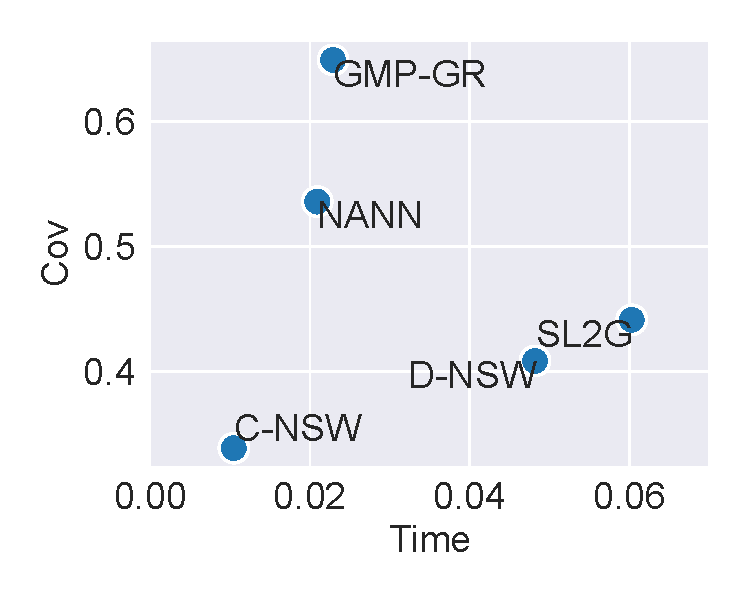
\includegraphics[width=0.47\linewidth]{figures/gmpgr/efficiency_Video.pdf}}
    \subfloat[MVideo]{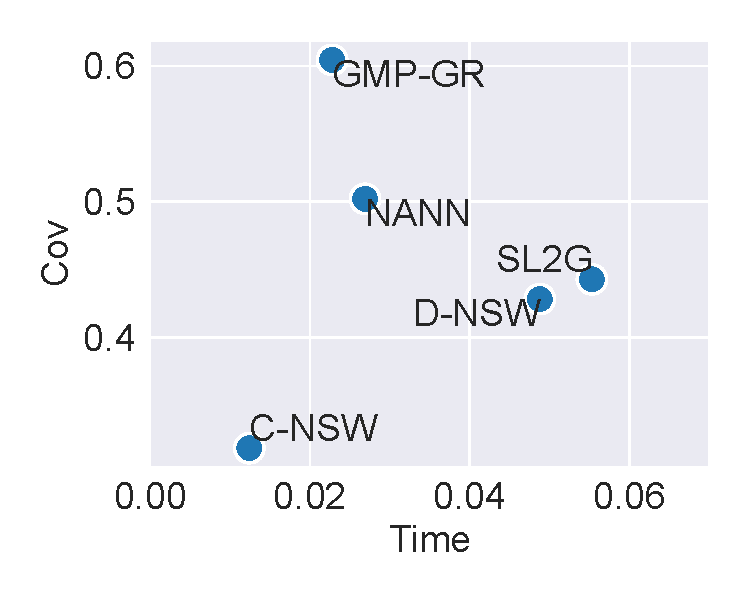
\includegraphics[width=0.48\linewidth]{figures/gmpgr/efficiency_MVideo.pdf}}
    \\[-0.5ex]
    \subfloat[Explore]{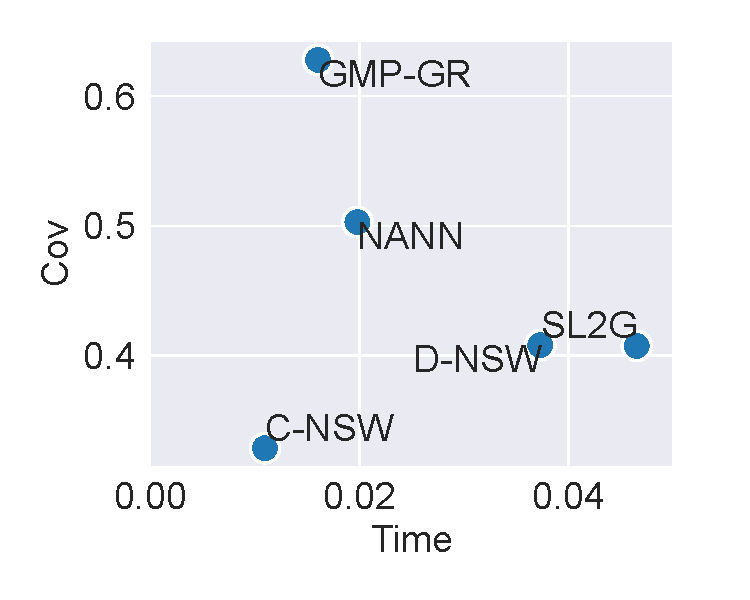
\includegraphics[width=0.47\linewidth]{figures/gmpgr/efficiency_Explore.pdf}}
    \subfloat[Fresh]{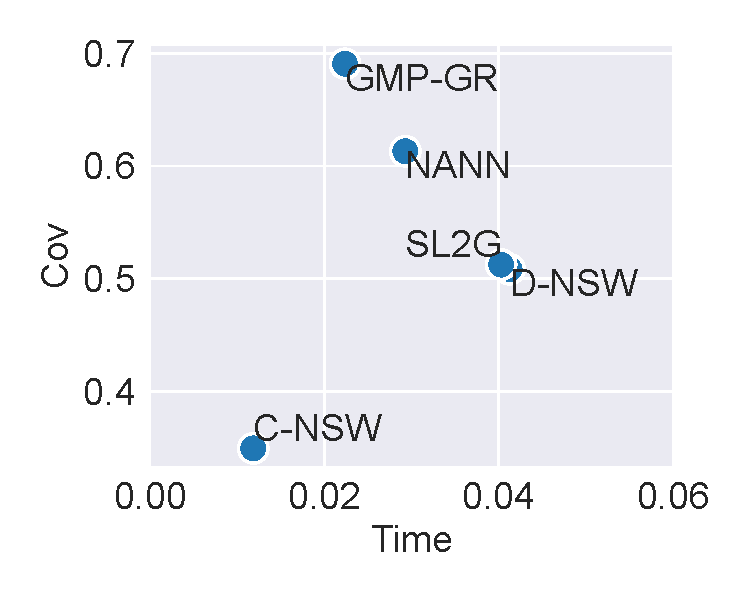
\includegraphics[width=0.47\linewidth]{figures/gmpgr/efficiency_Fresh.pdf}}
    \caption{Correlation between retrieval performance and efficiency on all four datasets. Methods closer to the upper-left corner achieve higher Cov with lower time cost.}
    \label{gmpgr:fig:efficiency}
\end{figure}

\paragraph{Ablation Study.}
We conduct an ablation study on GMP-GR in Figure~\ref{gmpgr:fig:ablation}, comparing it with two variants, \ie, GMP-GR-P and GMP-GR-M. The four panels jointly report Cov, retrieval speed, Rec@10, and Rec@100, allowing the effects on effectiveness and efficiency to be read together.
GMP-GR-P replaces MUIRML with a single supervision of the behavior in which a user visits an item, and GMP-GR-M substitutes HiPANNS with a standard HNSW search algorithm.
Specifically, we find that GMP-GR consistently outperforms both GMP-GR-P and GMP-GR-M across different datasets.
This superiority can be attributed to two key factors. First, MUIRML significantly enhances the relevance estimation accuracy and pathfinding efficiency. Second, HiPANNS prevents the graph-based ANNS process from succumbing to local optima by distributed and co-optimized search.
In addition, GMP-GR also shows a notable advantage in retrieval speed that replacing HiPANNS with a standard HNSW search algorithm can result in a great degradation of retrieval speed. This observation underscores the pivotal role of HiPANNS in acceleration. Furthermore, a more effective user-item relevance metric not only enhances the accuracy but also reduces traversal steps to converge to optimal candidates.

\begin{figure}[t]
    \centering
    \subfloat[Cov]{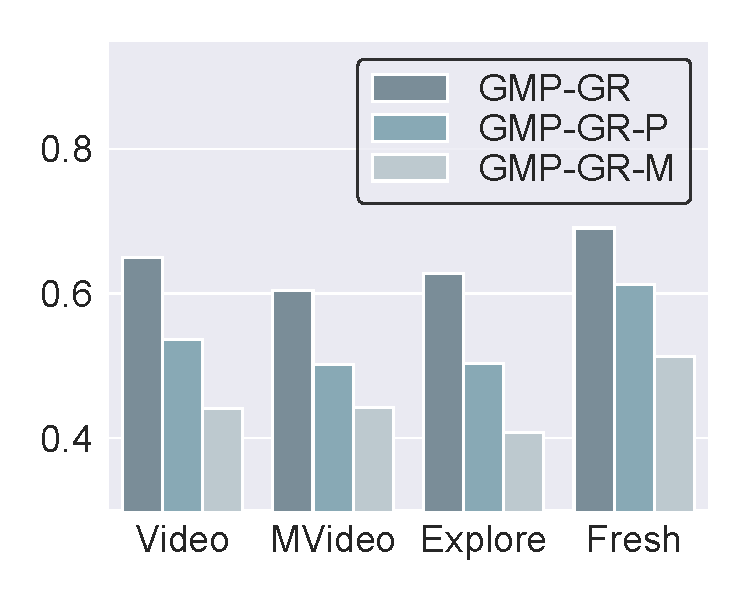
\includegraphics[width=0.42\linewidth]{figures/gmpgr/ablation_Cov.pdf}}
    \subfloat[Speed~($10^6$ items / sec)]{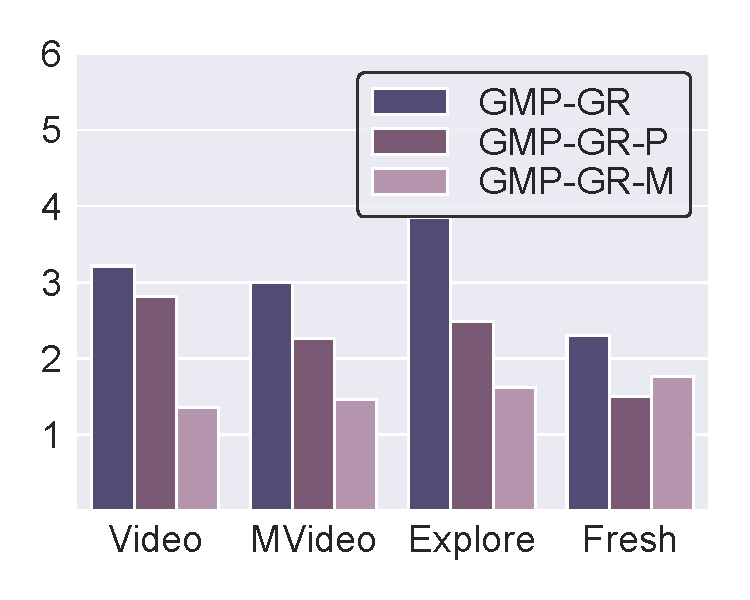
\includegraphics[width=0.42\linewidth]{figures/gmpgr/ablation_ItemPerS.pdf}}
    \\[-0.5ex]
    \subfloat[Rec@10]{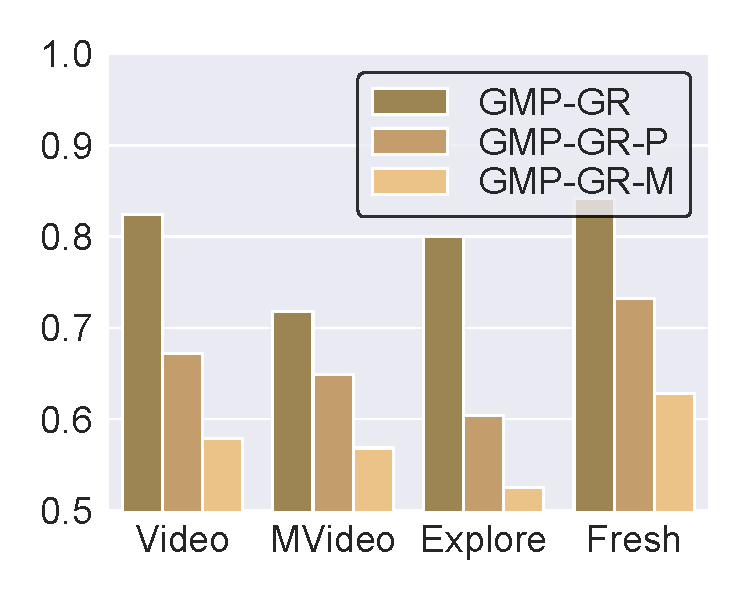
\includegraphics[width=0.42\linewidth]{figures/gmpgr/ablation_Rec10.pdf}}
    \subfloat[Rec@100]{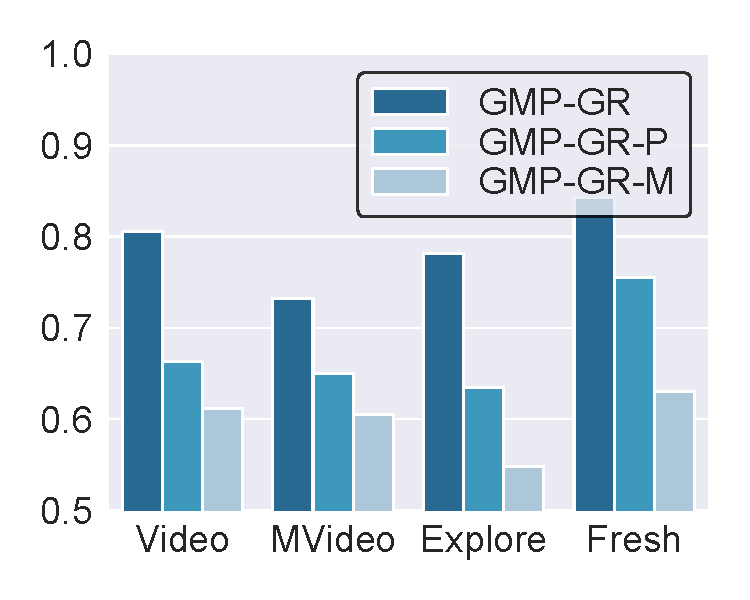
\includegraphics[width=0.42\linewidth]{figures/gmpgr/ablation_Rec100.pdf}}
    \caption{Ablation study of GMP-GR across retrieval effectiveness and efficiency metrics.}
    \label{gmpgr:fig:ablation}
\end{figure}

\FloatBarrier
\subsection{Online Testing}

We deploy GMP-GR in the Baidu Mobile APP for two services supported by five servers for online testing.
Service 1 is for the main recommendation list on the initial page.
Service 2 is for the next recommendation sequence that can be accessed after clicking on a video in immersive mode.

\subsubsection{Time on Page and Daily Active Users}

Table~\ref{gmpgr:tab:user_exp} depicts the impact of deploying GMP-GR on time on page and daily active users. Our results indicate a significant improvement in time on page and daily active users across the two services.
The integral components of GMP-GR, MUIRML, and HiPANNS, contribute to a $0.57\%$ and $0.23\%$ improvement in time on page, respectively.
Our findings suggest that the deployment of GMP-GR with improved modules has positively impacted user engagement and satisfaction.

\begin{table}[t]
    \caption{Online user statistics for two services.}
    \label{gmpgr:tab:user_exp}
    \centering
    \begin{tabular}{c|cc|cc}
        \toprule
        & \multicolumn{2}{c|}{Time on Page} & \multicolumn{2}{c}{Daily Active Users} \\
        & \textit{Service 1} & \textit{Service 2} & \textit{Service 1} & \textit{Service 2} \\
        \midrule
        GMP-GR & +1.13\% & +1.19\% & +0.23\% & +0.50\% \\
        \bottomrule
    \end{tabular}
\end{table}

\subsubsection{Query Throughput}
We also examine the query throughput influenced by the system acceleration strategies. The results demonstrate a strong improvement in query throughput, with an approximate doubling of throughput in the two services. Specifically, our analysis shows that the compilation optimization has led to a $74\%$ and $75\%$ increase in throughput by simplifying the computational graphs. Similarly, the model quantization has resulted in a $26\%$ and $25\%$ increase in throughput by decreasing DNN-based calculations. These findings underscore the effectiveness of GMP-GR in optimizing query processing and system efficiency.

\subsubsection{Statistical Analysis of Traffic and Latency}

\begin{figure}[t]
    \centering
    \subfloat[Traffic of two weeks in June, 2024.]{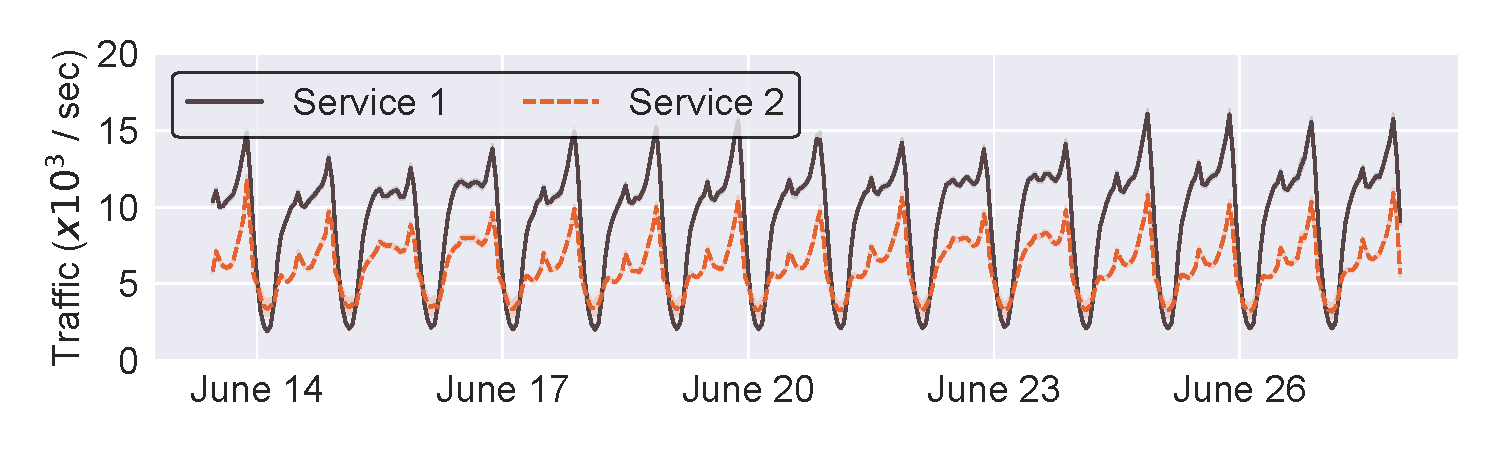
\includegraphics[width=\linewidth]{figures/gmpgr/timestamp_traffic.pdf}\label{gmpgr:fig:timestamp_traffic}}\\
    \subfloat[Latency in one day.]{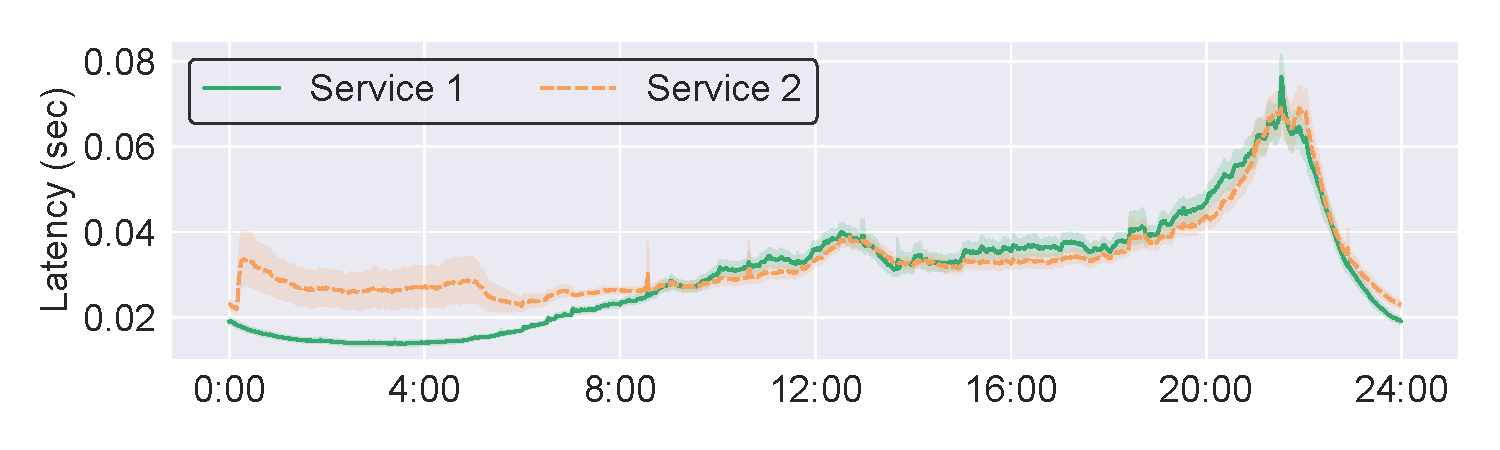
\includegraphics[width=\linewidth]{figures/gmpgr/timestamp_latency.pdf}\label{gmpgr:fig:timestamp_latency}}
    \caption{Temporal statistics of traffic and latency.}
    \label{gmpgr:fig:timestamp_traffic_latency}
\end{figure}

We collect traffic and latency statistics per second, which are recorded in a distributed manner at five servers in two services.
First, we examine the temporal patterns as shown in Figure~\ref{gmpgr:fig:timestamp_traffic_latency}. Specifically, Figure~\ref{gmpgr:fig:timestamp_traffic} illustrates the traffic trends over a two-week period, highlighting periodic fluctuations in query volumes. Meanwhile, Figure~\ref{gmpgr:fig:timestamp_latency} provides a more granular view of latency statistics over a 24-hour cycle, revealing variations in online response times in one day.
Moreover, we investigate the distributions of traffic and latency and explore their correlations in Figure~\ref{gmpgr:fig:service_traffic_latency}. The result indicates a direct relationship between query traffic and latency, with higher traffic volumes leading to longer response times. Furthermore, we observe distinct patterns in the latency-traffic relationships across five servers, reflecting divergence in computational resources and workload distribution.
Finally, Figures~\ref{gmpgr:fig:server_traffic} and~\ref{gmpgr:fig:server_latency} summarize the traffic and latency statistics across five servers, providing insights into the performance characteristics in terms of query processing and response times.

Taken together, the offline and online results show that search scaling cannot be reduced to faster graph traversal alone. Retrieval quality, navigation behavior, and GPU execution efficiency must be optimized jointly for the learned relevance signal to remain effective under production-scale traffic. This system-level evidence completes the progression from semantic representation through observational efficiency to large-scale search developed across the three technical chapters.

\begin{figure}[t]
    \centering
    \subfloat[Service 1]{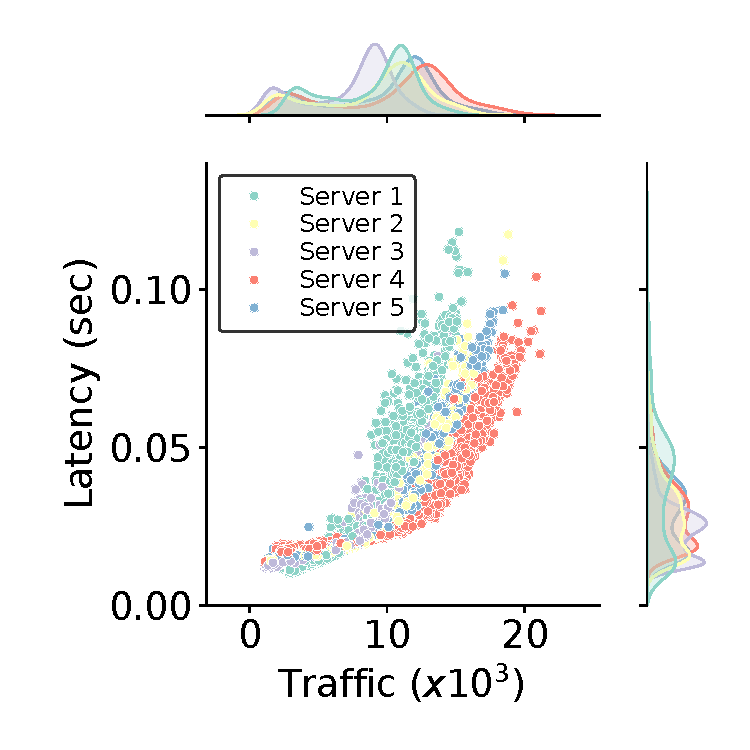
\includegraphics[width=0.38\linewidth]{figures/gmpgr/service_1_traffic_latency.pdf}}
    \hspace{0.04\linewidth}
    \subfloat[Service 2]{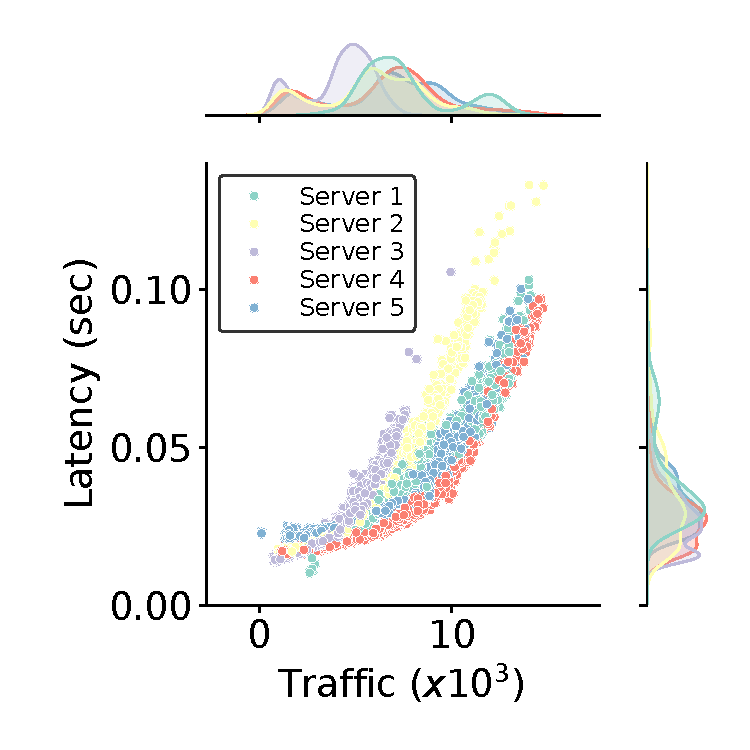
\includegraphics[width=0.38\linewidth]{figures/gmpgr/service_2_traffic_latency.pdf}}\\[-0.5ex]
    \subfloat[Traffic across servers]{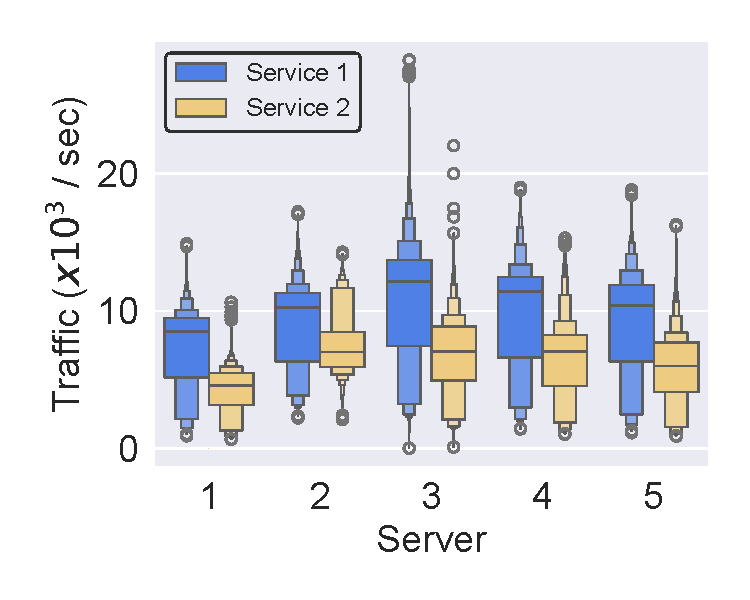
\includegraphics[width=0.38\linewidth]{figures/gmpgr/server_traffic.pdf}\label{gmpgr:fig:server_traffic}}
    \hspace{0.04\linewidth}
    \subfloat[Latency across servers]{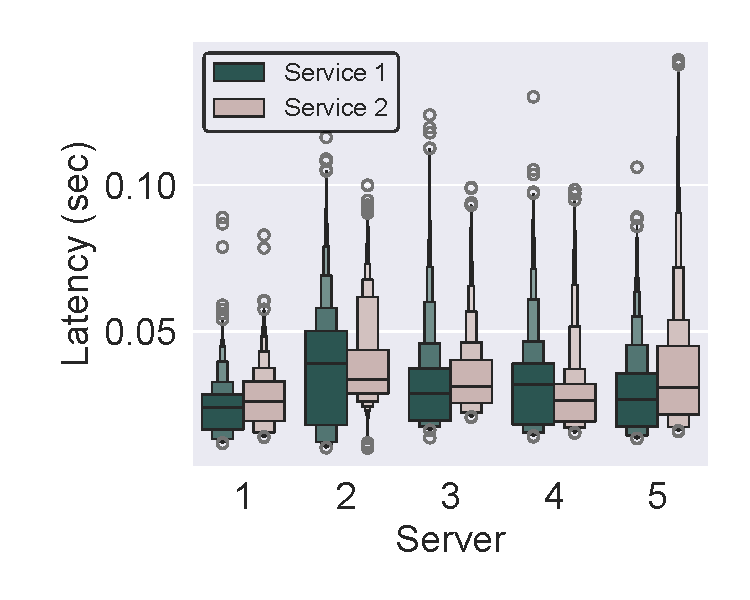
\includegraphics[width=0.38\linewidth]{figures/gmpgr/server_latency.pdf}\label{gmpgr:fig:server_latency}}
    \caption{Distributions and relationships of traffic and latency across two services and five servers.}
    \label{gmpgr:fig:service_traffic_latency}
\end{figure}

\FloatBarrier
\section{Chapter Summary}

This chapter addressed the search-scaling stage of the thesis by studying how a learned relevance signal can be used for accurate and efficient retrieval over web-scale recommendation collections. It introduced GMP-GR, which combines multi-relational user-item relevance metric learning with hierarchically parallel graph search and system-level GPU optimizations. Offline experiments showed consistent gains in retrieval quality and a favorable balance between accuracy and search speed. The ablation results attributed these gains to both MUIRML and HiPANNS. Online deployment further demonstrated improvements in user engagement and query throughput under production traffic.

Within the thesis, this chapter completes the progression from representation to deployment. Chapter~\ref{ch:universal-video-retrieval} established semantic generalization across retrieval tasks and domains, while Chapter~\ref{ch:spatiotemporal-scaling} studied how observational density affects the evidence preserved by video embeddings. The present chapter showed that these representations must also be paired with a relevance metric, graph-navigation strategy, and execution system that remain effective at large candidate scale. Together, the three studies position scalable video retrieval as a joint problem of semantic coverage, observational efficiency, and search-system efficiency.
